\documentclass{article}
\usepackage[margin=2cm]{geometry}
\usepackage{tabularx}
\usepackage{booktabs}
\usepackage{multirow}
\usepackage{enumitem}
\usepackage{url}
\usepackage{graphicx}
\usepackage{caption}
\usepackage{wrapfig}
\usepackage{setspace}
\usepackage{xcolor}
\usepackage{amsmath}
\usepackage{svg}
\usepackage{hyperref} % Required for hyperlinks
\usepackage{multicol} % this package is used to divide the document into multiple columns

\makeatletter
\renewcommand{\maketitle}{\bgroup\setlength{\parindent}{0pt}
\begin{center} % Center the title
  \Large\@title
  \newline
  \footnotesize\@author
\end{center}
\begin{flushright}
  \@date
\end{flushright}
\egroup}
\makeatother

% Adjust line spacing
\setstretch{0.9}

% Adjust paragraph spacing
\setlength{\parskip}{0pt}

\begin{document}

\title{Impact of Liquidity Pool Size on Trading Volume in BTC-ETH Pools}
\author{
  Team \#111 \\
   \scriptsize Matias Vizcaino (avizcaino3) | Walter Jack Simmons (wsimmons35) | MingShen Wang (mwang709) | Vítor de Matos Castilho (vcastilho3)
}
\date{09 July 2023}
\maketitle

\noindent
% {\setlength{\tabcolsep}{4pt} % Reduce column spacing


\section*{\textbf{Problem Statement and Objective}}

Decentralized Finance (DeFi), hosting about 48.78 billion USD in total value (as of April 23, 2023\cite{defillama}), relies heavily on liquidity pools in decentralized exchanges like Uniswap for efficient crypto trading. These pools, using an automated market maker model, earn from trading fees, participation rewards, and interest, distributed among liquidity providers based on their pool share\cite{Miori2022,Aigner2021,Xu2023}.

This study primarily \textbf{aims to examine the influence of pool size on trading volume, specifically in BTC-ETH liquidity pools in exchanges like Uniswap}. It hypothesizes a direct correlation between pool size and trading volume, supported by existing studies\cite{Miori2022,Heimbach2022}. Our study confirms a strong relationship between liquidity pool sizes and trading volumes in BTC-ETH pools, providing valuable insights for market participants and future research. This understanding could optimize liquidity provision, enhance DeFi market efficiency, and benefit stakeholders. For instance, liquidity providers could improve fee returns and risk management, traders could refine strategies, and DeFi platforms could develop more effective liquidity pools\cite{Makarov2022,Miori2023}.

\section{\textbf{Uniswap Liquidity Pools: An Overview}}

Various DeFi platforms cater to different needs. Uniswap, a popular choice, provides a user-friendly interface and a broad spectrum of token pairs. Other platforms like Curve Finance and Balancer offer low-slippage trades and customizable pools, respectively\cite{Xu2023}.

Uniswap, a decentralized exchange (DEX) on Ethereum, supports trading of Ethereum-native and wrapped non-native assets. It uses a Constant Product Market Maker (CPMM) model in which liquidity providers deposit two tokens, keeping a constant product of reserves\cite{Miori2023, Heimbach2022,Miori2023}.

Uniswap v3 introduced the concept of "virtual" versus "real" reserves, where virtual reserves behave as if all liquidity is concentrated at the current price range \cite{Elsts2021}. The unique mechanism allows more efficient capital usage and offers liquidity providers the ability to customize their price exposure. Precise calculations of position holdings and pool's parameters are possible through the equations provided by the Uniswap v3 liquidity math paper \cite{Elsts2021,Miori2023}. Uniswap V3's liquidity pools and the constant product market maker (CPMM) model are at the heart of the study of BTC-ETH pools. Research conducted in this area provides key insights and methodologies for predicting trading volume based on various activities within these pools \cite{Miori2023}. A detailed understanding of decentralized finance (DeFi) and how it differs from traditional financial structures is crucial in order to fully comprehend the mechanics of automated market makers (AMMs) and the operation of liquidity pools \cite{Makarov2022}

The CPMM formula is given by:

\[x \cdot y = k \quad \text{and} \quad price = \frac{y}{x}\]

Here, \(x\) and \(y\) denote the quantities of Token X and Y in the pool, and \(k\) is the constant product\cite{Makarov2022,Miori2023}.

Uniswap operates without a central authority, ensuring privacy, fund control, and a diverse range of tokens\cite{Miori2023}. Centralized exchanges (CEX), though offering faster transaction speeds and better customer support, may pose security risks as they hold user funds\cite{Makarov2022}. Liquidity pools in DEXs enable direct interaction with smart contracts, ensuring continuous liquidity but exposing liquidity providers to impermanent loss risks\cite{Aigner2021, Heimbach2022}. Prices are influenced by trade size, market conditions, supply-demand dynamics, and external price changes\cite{Miori2022,Heimbach2022,Miori2023}.

\section{\textbf{Analytical Methodology}}

A thorough analysis of the interconnectedness between Uniswap v3 pools and a systematic selection of subsets of pools for analysis is required. This will be done over different time periods, using similar methodologies as found in recent studies \cite{Miori2022}. The relationship between liquidity, trading volume, and price stability in pools will be examined, along with an investigation of how liquidity pool size impacts trading volume.

\begin{table}[htbp]
  \centering
  \small
  \begin{tabularx}{\linewidth}{|>{\raggedright\arraybackslash}X|}
  \hline
  \textbf{Feature Engineering:} Our models' predictive power was enhanced by creating new features from existing data\cite{Miori2023}. This process effectively captured crucial information about liquidity pool dynamics, spillover effects, and price divergences. \\
  \hline
  \textbf{Modelling and Optimization:} Through the application of Ordinary Least Squares (OLS) regression, we examined the relationship between liquidity pool size and trading volume, which offered profound insights into their interplay\cite{Miori2023}. Model performance was assessed using metrics such as R-squared, while we optimized feature selection, corrected multicollinearity, and explored alternative functional forms for improved model accuracy and interpretability\cite{Miori2023}. \\
  \hline
  \textbf{Innovations:} Building on the reference paper, we implemented the underlying code in Python, thus creating a robust data model to explore interactions between two liquidity pools more effectively\cite{Miori2023}. Furthermore, we developed a mathematical language to facilitate the data engineering aspects of the data model\cite{Miori2023}. \\
  \hline
  \end{tabularx}
  \caption{Analytical Techniques and Main Contributions}
  \label{fig:analytical-techniques}
  \end{table}
  
  Substantial accomplishments were achieved at each of our research stages, leading to a robust analysis and valuable results\cite{Miori2023}.

  \begin{table}[htbp]
  \centering
  \small
  \begin{tabularx}{\linewidth}{|>{\raggedright\arraybackslash}X|}
  \hline
  \textbf{Data Collection:} We sourced data from multiple APIs (Uniswap, Binance) successfully, and associated this data with Ethereum block numbers for consistent time measurement. \\
  \hline
  \textbf{Data Preprocessing:} We maintained data consistency, addressed discrepancies from different sources, and efficiently cleaned, formatted, and handled missing values in the dataset. \\
  \hline
  \textbf{Exploratory Data Analysis (EDA):} Utilizing EDA, we generated descriptive statistics, visualizations, and correlation analyses. This approach facilitated the identification of trends, outliers, and the relationships between variables. \\
  \hline
  \textbf{Final Analysis and Conclusions:} We articulated our findings and conclusions, providing quantitatively-driven insights with the potential to enhance liquidity provision, optimize trading strategies, and improve the efficiency of DeFi marketplaces. \\
  \hline
  \textbf{Confirmation of Results:} Our results largely coincide with those in the reference paper, with minor discrepancies likely due to the techniques used and features available. Notably, we utilized fewer features and feature categories than the reference paper, which might explain the minor divergences observed in our results\cite{Miori2023}. \\
  \hline
  \end{tabularx}
  \caption{Supporting Work and Confirmation of Results}
  \label{fig:approach-accomplishments}
  \end{table}

Our work provides a significant contribution by offering an open framework that allows other researchers and professionals to conduct further research in this field. This outcome not only answers our problem statement but also opens avenues for future exploration\cite{Miori2022}.

\subsection{\textbf{Challenges and Insights}}

Our main challenges were data collection and processing due to intricate engineering and the rate limits of the Etherscan free-tier API\cite{etherscanAPI}. Nonetheless, we overcame these hurdles and made significant progress in understanding liquidity pool dynamics\cite{Miori2022,Aigner2021,Miori2023}.

We embraced two time concepts—"trading clock" and "time horizon"—which enabled us to thoroughly explore both short and long-term trends. This detailed analysis offered invaluable insights for decision-making and risk management in the DeFi ecosystem\cite{Miori2022}.

We successfully addressed complexities in understanding entry-level liquidity pool mathematics and integrated the associated formulas into calculations.py functions. This step significantly enriched our feature derivation and bolstered our overall analysis\cite{Elsts2021,Aigner2021}.
For instance, we tackled the complexity of tick math, which involves mapping discrete ticks to continuous prices. This step, guided by the Uniswap v3 liquidity math paper, was essential for interpreting Uniswap data and indexes \cite{Elsts2021}. In addition, we adjusted raw price ratios for token decimals to get human-readable prices, a process critical for presenting our analyses \cite{Elsts2021}.

\textbf{Key Note:} Our models and code implementation have been designed with a focus on programming and data structure, and while they provide valuable insights, further improvement is needed to enhance the accuracy and completeness of our results. We encourage peer review and rigorous testing of our calculations.py module, as well as a deeper understanding of the underlying liquidity mathematics as outlined in the Uniswap v3 liquidity math paper \cite{Elsts2021,Miori2023}.

\section{\textbf{Engineering Ecosystem}}

Data engineering and feature extraction are crucial elements for building robust predictive models. In the case of analyzing BTC-ETH trading volume on Uniswap, several aspects of data must be considered.

First, let's consider the nature of the data we are dealing with. Uniswap is a decentralized exchange that operates on an automated market-making (AMM) model, and its Version 3 (v3) utilizes a novel mechanism of concentrated liquidity pools. The structure and dynamics of these liquidity pools play a crucial role in trading volumes \cite{Miori2023}. We must extract relevant data from these pools, including their sizes, trading volumes, and related metrics, for accurate analysis. Understanding DeFi's goals and mechanisms from a broad perspective is also valuable \cite{Makarov2022}.

Moreover, it's important to incorporate data from different sources, considering not just the pools of interest but also neighboring pools and other prominent exchanges such as Binance. This kind of broad-spectrum data helps in capturing spillover effects, which are significant drivers of trading volume \cite{Miori2023}. For example, we can study the effects of trading volume and the activities from interconnected DeFi protocols and stablecoins \cite{Miori2022}.

Feature selection is a crucial part of the process. Stepwise regression can be an effective tool for optimizing the model and refining the set of independent variables \cite{Miori2023}. We should also account for factors like network effects, economies of scale, and concentration issues that can influence liquidity provision \cite{Makarov2022, Miori2022}.

From a risk perspective, we should account for external risks to liquidity providers like arbitrage opportunities, fraudulent DEXs, regulatory risks, censorship risks, etc. \cite{Aigner2021}. Systemic risks from interconnected DeFi protocols and stablecoins could also impact trading activity \cite{Makarov2022}. Additionally, economic risks like yield dilution, conversion risk, exchange risk, counterparty risk, and liquidation risk pose challenges and should be considered \cite{Xu2023}.

For the implementation part, we can take advantage of mathematical equations and formulations. For example, we can use equations to calculate the amounts of assets based on liquidity, price range, and the current price \cite{Elsts2021}. Formulas for calculating impermanent loss and changes in holdings after a price change could also be useful in our analysis \cite{Elsts2021, Aigner2021, Heimbach2022}.

\subsection{\textbf{Dataset}}

In line with the \textit{"DeFi modeling and forecasting trading volume" (2023)} study\cite{Miori2023}, we gathered and structured trade data spanning a minimum of 6 months. Our GitHub repository provides more details and the code used to gather this information\cite{TeamRepo}. Our dataset incorporates information from the following sources:

\begin{table}[ht]
  \centering
  \small
  \begin{tabular}{|p{0.15\linewidth}|p{0.35\linewidth}|p{0.5\linewidth}|}
  \hline
  \textbf{Source} & \textbf{Description} & \textbf{Data} \\
  \hline
  Uniswap's The Graph API\cite{uniswapAPI} & This API offers transaction details, trading volumes, and block data from Uniswap v3 liquidity pools. & Includes transaction IDs, timestamps, amounts, USD equivalents, and other related data. \\
  \hline
  Etherscan API\cite{etherscanAPI} & Utilized to extract corresponding transaction data from Etherscan based on transaction hashes. & Block hashes, block numbers, sender addresses, gas details, transaction hashes, and other relevant information. \\
  \hline
  Binance\cite{binanceData} & Provides Centralized Exchange (CEX) data for ETHBTC trades. Data was obtained via scripts from Binance's GitHub repository. & Contains detailed data about each trade performed on the Binance platform, including trade prices, quantities, timestamps, and buyer/seller characteristics. \\
  \hline
  \end{tabular}
  \caption{Dataset Source Description}
  \label{tab:dataset-description}
  \end{table}

\subsection{\textbf{Key Variables}}

\textbf{Target Variable:} The key dependent variable in our study is the trading volume of liquidity pools (amountUSD) over specific blocks. We propose several models for different time horizons to investigate how the relationships evolve over time.

\textbf{Independent Variables:} Constructed from various features and are grouped as follows:

\begin{enumerate}[label=\arabic*. ,itemsep=0pt, topsep=0pt]
\item \textbf{Direct Pool Features (41):} Measures such as volatility, rate, number of trades, and average trade size.
\item \textbf{CEX Spillover Effects (6):} Variables like actual coin trade volume on Centralized Exchanges (CEX), which can influence liquidity pools on decentralized platforms.
\end{enumerate}


\section{\textbf{In-Depth: Feature Engineering}}

Feature engineering is key in deciphering the intricate dynamics between variables in our analysis, with particular focus on historical patterns in the Decentralized Exchange (DEX) pools and the influence of Centralized Exchange (CEX) activities.

Initially, we define all blocks within our analysis scope. Subsequently, we establish the Reference blocks, followed by determining the interval between reference blocks, encompassing all blocks within this range.

Let's symbolize the entire sequence of blocks within our analysis scope as $B$ and denote the total number of blocks under scrutiny as $K$. We can represent this in the following manner:

\begin{equation}
B = \{b_k\}_{k=1}^{K} \text{ where each } b_k \text{ is a block within the scope of analysis}
\end{equation}

In the construction of a time-series data model, the "Reference Block" serves as a time marker. These blocks, identified by Mint Operations, act as pivot points within the blockchain when users infuse liquidity into different pools on the DEX, such as Uniswap. Since we aim to study the iteraction and effects within and across pools, the Reference Blocks are further classified into "same" and "other" pools, arranged in reverse chronological order, with the latest block placed at the top and assigned an index of 0.

\begin{equation}
R_{s} = \{b_{s}\}_{s=1}^{S} \text{ where each } b_{s} \text{ is a block in } B \text{ and serves as a reference block in the "same" pool}
\end{equation}

\begin{equation}
R_{o} = \{b_{o}\}_{o=1}^{O} \text{ where each } b_{o} \text{ is a block in } B \text{ and serves as a reference block in the "other" pool}
\end{equation}

Here, $S$ and $O$ represent the total count of reference blocks in the "same" and "other" pools respectively.

The intervals between these reference blocks can be represented as a sequence of block numbers between $b_i$ and $b_j$ (including $b_i$). This is defined as:

\begin{equation}
I = \{b_{ij}\}_{\substack{i=0,j=i+1 \ i,j\leq N}}^N
\end{equation}

Here, $b_{ij}$ refers to the sequence of blocks from $b_i$ to $b_{j-1}$, including $b_i$ but excluding $b_j$, accurately encapsulating the concept of an interval.

Block Reference Interval chains derived from the "same" and "other" pools' mint operations generate sequences of block numbers, encompassing the last N reference blocks and every block between them, where N denotes the number of lags or intervals assessed for the direct features. We denote these chains of "same" and "other" pools as $C_{s}$ and $C_{o}$ respectively, and they can be defined as follows:

\begin{equation}
C = \{b_{i}\}_{i=0}^{N} \text{ where each } b_{i} \text{ is a block} \in \{R_s, R_o\} \text{ and } b_{i} > b_{i+1} \text{ for } i \in \{0,1,...,N-1\}
\end{equation}

Future periods, or time horizons, are constructed for predictions or analyses of target variables by commencing from the first Reference Block and incrementing the block count by M until the succeeding reference block is reached. Here, M signifies the number of blocks or periods between reference points, shaping the construction of the dependent variable. The optimal choice of M determines the time horizon length and granularity, impacting the analysis' detail level and prediction accuracy.

\begin{equation}
H_{M} = \{b_{0}+kM\}_{k=0}^{K} \text{ with } K = \min \left( K_{\text{max}}, \left\lfloor \frac{\text{distance to next reference block}}{M} \right\rfloor \right)
\end{equation}

\begin{figure}[htbp]
  \begin{minipage}{0.5\textwidth}
  \centering
  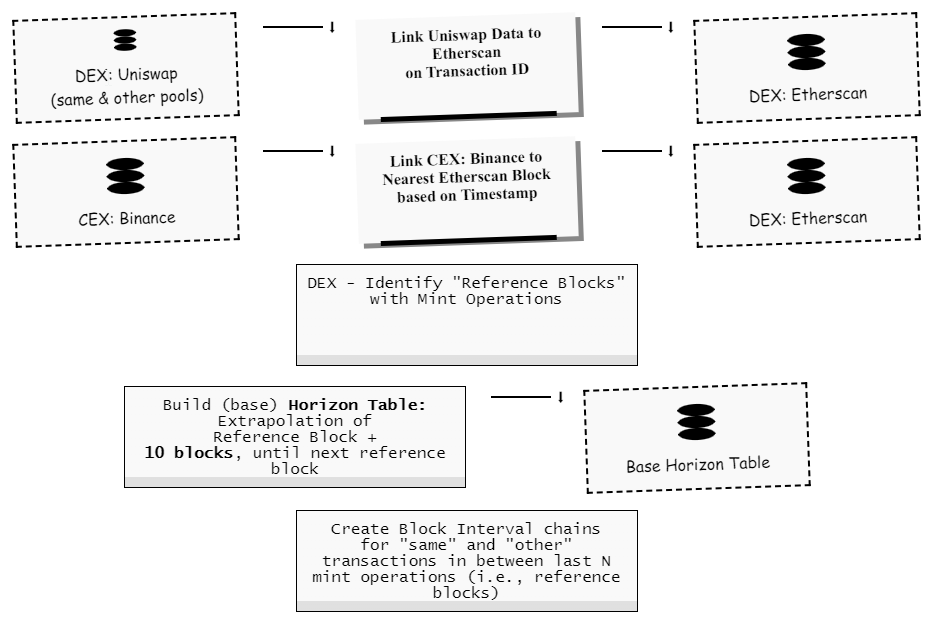
\includegraphics[width=\linewidth]{C:/Users/MatiasVizcaino/repos/6203-DataAnalyticsBusiness-Project/Other Resources/data-diagram/engineer.png}
  \caption{Data Engineering}
  \label{fig:data-diagram-engineer}
  \end{minipage}
  \begin{minipage}{0.45\textwidth}
  \centering
  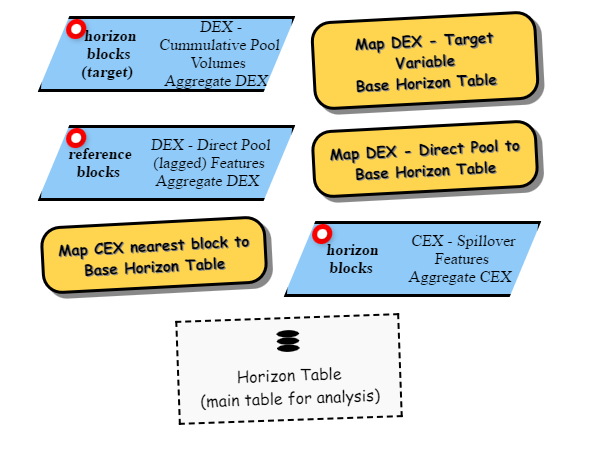
\includegraphics[width=\linewidth]{C:/Users/MatiasVizcaino/repos/6203-DataAnalyticsBusiness-Project/Other Resources/data-diagram/features.png}
  \caption{Feature Engineering}
  \label{fig:data-diagram-features}
  \end{minipage}
  \end{figure}

The Horizon Block Table encapsulates the dynamics and relationships between the "same," "other," and "both" pools by assessing their respective target variables and features at different horizons and lags. The granularity level varies for each component within the Horizon Block Table, as illustrated in the following table:

\begin{equation}
HBT = \{ (H_{M}, F_{\text{DEX}}, F_{\text{DP}}, F_{\text{CEX}}) \} \text{ for each horizon } H_{M} 
\end{equation}

\begin{table}[htbp]
\centering
\begin{tabular}{|c|c|}
\hline
\textbf{Component} & \textbf{Granularity Level} \\
\hline
DEX target variable & Horizon block level \\
\hline
DEX direct pool features & Reference block level \\
\hline
CEX spillover features & Horizon block level \\
\hline
\end{tabular}
\caption{Granularity Level of Components in Horizon Block Table}
\label{table:granularity}
\end{table}

This granularity distinction enables a comprehensive examination of the "same" and "other" pool behaviors and interactions at various levels within the time-series data model. The Horizon Block Table illuminates the data dynamics, unraveling the cooperative or competitive dynamics between the "same" and "other" pools over the time series.

\section{Data Profiling Report}
Our data profiling report details our analyses concerning block intervals, transaction types, reference blocks, and target variables. This examination aids in establishing a comprehensive understanding of our dataset, facilitating robust model fitting and further analysis.

The merging process of Uniswap transactions and Etherscan data showed a high match rate of transactions for the six-month analysis period, validating our dataset's integrity. Additional cleaning and integrity checks were carried out on each data source to aid future processing.

\subsection{Block Intervals and Transactions}
The dataset comprises block intervals ranging from 0 to 3, with block time representing the number of blocks between reference blocks that carry out a mint operation in both "same" and "other" pools. A pattern of increasing block time and transaction count is observed as we move from recent to preceding intervals. 

Transactions are classified into 'burns', 'mints', and 'swaps', with 'swaps' being the most common transaction type across all dates and pools. The volume of each transaction type varies over time, indicating market dynamics. 

\subsection{Reference Blocks}
Reference blocks form a critical component in our analysis. Our dataset accommodates different numbers of reference blocks for the 500 (3,242 transactions) and 3000 (4,986 transactions) pools, with each block serving as a reference point for recording block time and transaction count. An unusual surge in mint activity recorded in July 2022 merits further investigation to uncover potential market influences or events during that period [TODO-Appendix]

\subsection{Target Variables}
The target variables in our dataset comprise 'cum\_volume\_500', 'cum\_volume\_3000', and 'cum\_volume\_base' for the 500, 3000, and both reference pools, respectively. These variables encapsulate cumulative volumes across different pools and underpin our forthcoming modeling and analysis.

\subsection{Data Cleaning and Preprocessing}
Prior to the modeling phase, it was essential to address records with missing values in the independent variables. Specifically, we identified null values in the volatility (same pool) and avg-USD/rate-USD (other pool) metrics. We deployed Python utility functions customized for Pandas DataFrame to conduct the initial data cleaning and preprocessing. These tasks comprised identifying and addressing missing values, eliminating correlated columns, and aggregating data at specific intervals.

\begin{itemize}
    \item \textbf{Handling Missing Values:} [CHECK THIS SECTION] Certain columns such as 'rate-USD-iother\_01', 'avg-USD-iother\_01', 'vol\_0\_1', 'vol\_0\_2', 'vol\_0\_3' contained null values, which we replaced with zeros to render the dataset suitable for model fitting.
    \item \textbf{Correlated Features:} We identified columns such as 'blsame\_2', 'blsame\_3', 'blother\_2', 'blother\_3', 'vol\_0\_1', 'vol\_0\_2' as highly correlated, leading to their removal from the dataset to prevent multicollinearity during model fitting.
    \item \textbf{Column Aggregation:} We aggregated certain columns that shared prefixes like 'rate-count-isame\_', 'rate-count-iother\_', 'binance-btc-', summing up their data in new columns appended with '03'. We subsequently dropped the original columns.
    \item \textbf{Data Loss Assessment:} We meticulously tracked the change in row count during the data cleaning process, which led to an insignificant data loss of 0.09\% observations, denoting a successful data cleaning operation with the majority of the data preserved.
\end{itemize}

\subsection{Data Preparation for Model Fitting}
We prepared three Horizon Tables (refbase, ref500, ref3000) for each mint of reference, leading to a total of 118,785 horizons. Before proceeding to fit the Ordinary Least Squares (OLS) models, we limited the horizons to a maximum of 30, which with K=10 it corresponds to about 300 blocks and $\sim$2.3 minutes (given a mean block time of 14 seconds). This step allows us to focus on the most immediate blocks, thereby reducing noise and enhancing the robustness of our modeling process.

% add new line
In conclusion, our detailed data profiling has enabled us to unearth critical insights into block intervals, transaction types, reference blocks, and target variables. Despite certain challenges such as missing values and high correlation among variables, strategic management of these issues ensures minimal data loss. This thorough comprehension of our data lays a robust foundation for the subsequent stages of our data exploration and analysis pipeline.


\section{\textbf{In-Depth: Modelling Approach}}

We are studying the correlation between the size of liquidity pools and trading volume using Ordinary Least Squares (OLS) regression models. The OLS method is favored due to its simplicity, interpretability, and widespread use in econometric analysis. Despite other models like Poisson regression, negative binomial regression, and logistic regression being available, they are more fitting for count data or binary outcomes, not our continuous outcome of interest. Plus, OLS aligns our research with other academic works\cite{Miori2023}, essential for the scarcity of research in this area.

The application of OLS to time-series models involves addressing temporal elements like time trends and seasonal patterns. However, OLS can still be used if our time-series data is believed to follow a linear trend, while considering issues such as autocorrelation and non-stationarity.

\subsection{\textbf{Model Construction and Evaluation}}

We define a set of pools, denoted as \(P\), where \(p \in P=\{500,3000,\text{both}\}\). This allows for individual, interaction, and aggregate metrics within and across two pools, enabling a comprehensive study and insights into spillover effects. 

A reference pool \(P_r\) is introduced, with \(P_r \in P\) and \(P_r \neq \text{both}\), denoting a pool where a reference mint operation occurs. This results in \(len(P) * len(P_r)\) possible combinations (i.e., 3*2=6).

The response variable in our model, \(Y_{p_{\text{horizon}}}\), denotes the cumulative volume for a pool at a given horizon. The explanatory variables are structured to discriminate "same" and "other" pool features using Block Interval Chains which were derived from the feature engineering process.

In particular, we use the sequences of block numbers generated by the chains for the "same" and "other" pools' mint operations, denoted \(C_s\) and \(C_o\) respectively, to define the explanatory variables \(X\). 

To incorporate temporal dependencies and dynamics in the model, we introduce spot lagged variables of the explanatory variables. These spot lagged variables, denoted as \(\widetilde{i(i-1)}X_s\) and \(\widetilde{i(i-1)}X_o\), represent the values of the explanatory variables at different lags relative to the prediction horizon, for the "same" and "other" pools respectively.

We stadarize the independent variables to make the fitted coefficients easier to compare to each other, because they're all on the same scale. For example, a coefficient of 0.5 means that a one standard deviation increase in the corresponding feature leads to a 0.5 increase in the predicted dependent variable, assuming all other variables are held constant.

Further, as described in Section \ref{sec:model-optimization}, we opt to perform a logarithmic transformation using base 10 on the response variables, similar to the approach outlined in \cite{Miori2023}.

The OLS regression model used in our study is expressed as follows:

\begin{equation}
  \log(Y_{p_{\text{horizon}}}) = \beta_0 + \sum_{i=1}^{n} \left(\beta_i^s \cdot \widetilde{i(i-1)}X_s + \beta_i^o \cdot \widetilde{i(i-1)}X_o\right) + \sum_{j=1}^{m} \beta_{n+j} \cdot X_j + \epsilon
  \end{equation}
  
  \begin{table}[h!]
    \centering
    \begin{tabular}{|c|p{0.6\linewidth}|}
    \hline
    \textbf{Variable} & \textbf{Definition} \\
    \hline
    \(\log(Y_{p_{\text{horizon}}})\) & Logarithm of the dependent variable to be predicted at the prediction horizon \(p_{\text{horizon}}\) \\
    \(\beta_0\) & Intercept term: Expected value of \(\log(Y_{p_{\text{horizon}}})\) when all variables are zero \\
    \(\widetilde{i(i-1)}X_s\), \(\widetilde{i(i-1)}X_o\) & Spot lagged variables: Values of \(X\) at different lags relative to the prediction horizon for the "same" and "other" pools, respectively \\
    \(\beta_i^s\), \(\beta_i^o\) & Coefficients associated with each spot lagged variable of \(X\), capturing their effects on the predicted value of \(\log(Y_{p_{\text{horizon}}})\) \\
    \(X_j\) & Additional independent variables or non-lagged variables of \(X\) included in the model \\
    \(\beta_{n+j}\) & Coefficients associated with each additional independent variable, indicating their effects on \(\log(Y_{p_{\text{horizon}}})\) \\
    \(\epsilon\) & Error term or residual: Accounting for unexplained variation in \(\log(Y_{p_{\text{horizon}}})\) not captured by the model \\
    \hline
    \end{tabular}
    \caption{Variable definitions}
    \label{tab:variables}
  \end{table}

We trained and evaluated models for different target variables and horizons, incorporating lagged variables to predict trading volumes at various time horizons. Model performance was assessed using several metrics.

\begin{table}[h!]
  \centering
  \begin{tabular}{|p{0.35\linewidth}|p{0.55\linewidth}|}
  \hline
  \textbf{Metric} & \textbf{Purpose} \\
  \hline
  R-squared & Represents the proportion of the variance for a dependent variable that's explained by an independent variable \\
  Adjusted R-squared & Adjusts the R-squared for the number of predictors in the model \\
  Mean Absolute Error (MAE) & Measures the average magnitude of the errors in a set of predictions \\
  Mean Squared Error (MSE) & Measures the average of the squares of the errors \\
  Root Mean Squared Error (RMSE) & Square root of the MSE, measuring the standard deviation of residuals \\
  \hline
  \end{tabular}
  \caption{Evaluation metrics}
  \label{tab:metrics}
  \end{table}  

\subsection{Train/Test Split and Cross-Validation}

The Train/Test Split methodology assessed the model's ability to generalize to unseen data. Our data set was partitioned into a training set for model training and a test set for evaluating predictive performance.

Cross-validation was applied to assess the OLS model for each horizon. We employed GroupKFold, a form of k-fold cross-validation, to prevent data leakage between training and testing sets. This ensured groups were not split between these sets. We defined groups according to the block reference number. For each fold, the data was split, features standardized, target variables transformed, and an OLS regression model fitted. R-squared and adjusted R-squared were computed for both training and test sets. This process was repeated for each horizon, resulting in trained models and performance metrics. Cross-validation aids in estimating model performance, identifying overfitting, and ensuring reliable generalization across different data subsets.

\subsection{Model Optimization}\label{sec:model-optimization}

Model training involved an iterative "All Horizon Runs" (as in Figure \ref{fig:ols-all-horizons}) approach to explore different modeling techniques, followed by a "Best Horizon Run" to optimize models based on performance. We used the coefficient of determination, R-squared, to gauge model performance, ensuring the model was well-specified and likely to generalize well to new data. 

\begin{figure}[htbp]
  \centering
  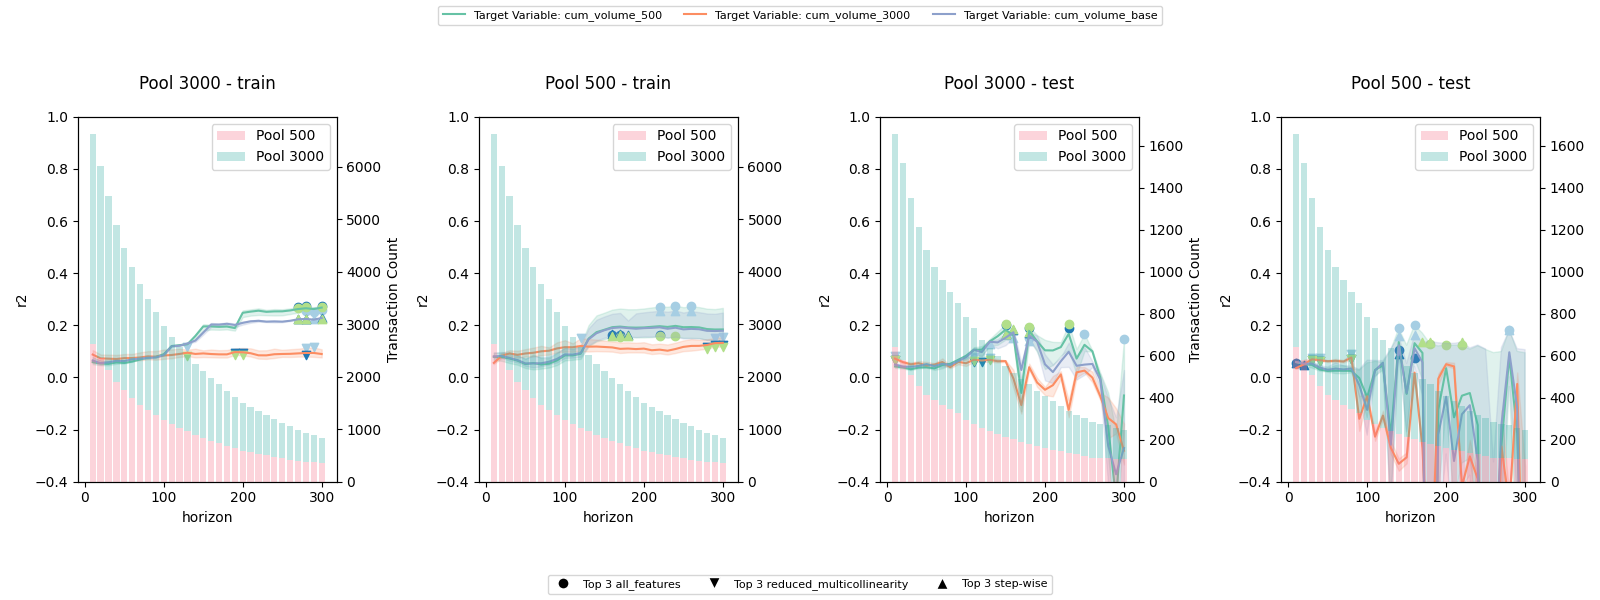
\includegraphics[trim=0 0 0 0, clip, width=\linewidth]{C:/Users/MatiasVizcaino/repos/6203-DataAnalyticsBusiness-Project/Other Resources/OLS_allhorizons_r2.png}
  \caption{OLS Horizon Analysis}
  \label{fig:ols-all-horizons}
\end{figure}

The coefficient of determination, also known as R2 score, quantifies the amount of variance in the dependent variable predictable from the independent variable(s). It ranges from 0 to 1, where 0 means the model explains none of the response data's variability around its mean, and 1 means it explains all the variability. However, R2 can be negative when the model fits poorly and performs worse than a horizontal line (the mean of the dependent variable). This may occur when the model's predictions are consistently far off, causing large errors, or when overfitting occurs on the training data, resulting in poor performance on the test data.

Our iterative "All Horizon Runs" and "Best Horizon Run" approaches allowed us to explore different modeling techniques and optimize the models based on performance. The results informed the selection of the most suitable models for predicting the target variables.

The "Best Horizon Run", focused on identifying the optimal model for specific combinations of horizon and target variables. The 'step-wise' model with parameters \texttt{pool = 3000} and \texttt{target\_variable = 'cum\_volume\_500'} outperformed others in both training and testing environments. We concentrated on \texttt{horizon = 150}, which displayed higher mean $R^2$ values of 0.203 in both training and testing data, indicating superior generalization and predictive accuracy. Other models, in contrast, yielded lower mean $R^2$ values, with some even producing negative values in the testing data, indicating suboptimal performance and poor generalization to unseen data.

The small differences between \(R^2\) and \(R^2_{adj}\) for both the overall data and the specific combination suggest that the 'step-wise' model is not overfitting due to the inclusion of too many predictors. This is a positive indication that the model is well-specified and likely to generalize well to new data. This supports the selection of the 'step-wise' model for the specific combination of parameters, as the model appears to have a good balance between complexity (number of predictors) and performance (as measured by \(R^2_{adj}\)).

In order to manage multicollinearity, we performed a correlation analysis and calculated the Variance Inflation Factor (VIF) as per the equation:

\begin{equation}
  VIF(k) = \frac{1}{1 - R^2_k}
\end{equation}

with $R^2_k$ being the determination coefficient for each predictor.

The condition \( \text{VIF} < b \) compares the Variance Inflation Factor (VIF) to a threshold value \( b \), where values less than 1 indicate low or no multicollinearity, values between 1 and 5 suggest moderate multicollinearity, and values greater than 5 indicate high multicollinearity.

\begin{table}[h]
\centering
\begin{tabular}{lcc}
\hline
 b & \textbf{Before Reduction} & \textbf{After Reduction} \\
\hline
\textbf{No/Low} & 0 & 0 \\
\textbf{Moderate} & 21 & 24 \\
\textbf{High} & 22 & 2 \\
\hline
\end{tabular}
\caption{VIF Counts for Thresholds [1, 5, inf]}
\end{table}

Two variables ('rate-count-iother', 'blother\_1') remained with high VIF. Following a correlation analysis, certain highly correlated features were removed. Further reduction of multicollinearity was achieved by aggregating certain intervals, a methodology based on \cite{Miori2023}. See Figure~\ref{fig:correlation-matrix} for the correlation matrix.

\begin{figure}[htbp]
  \centering
  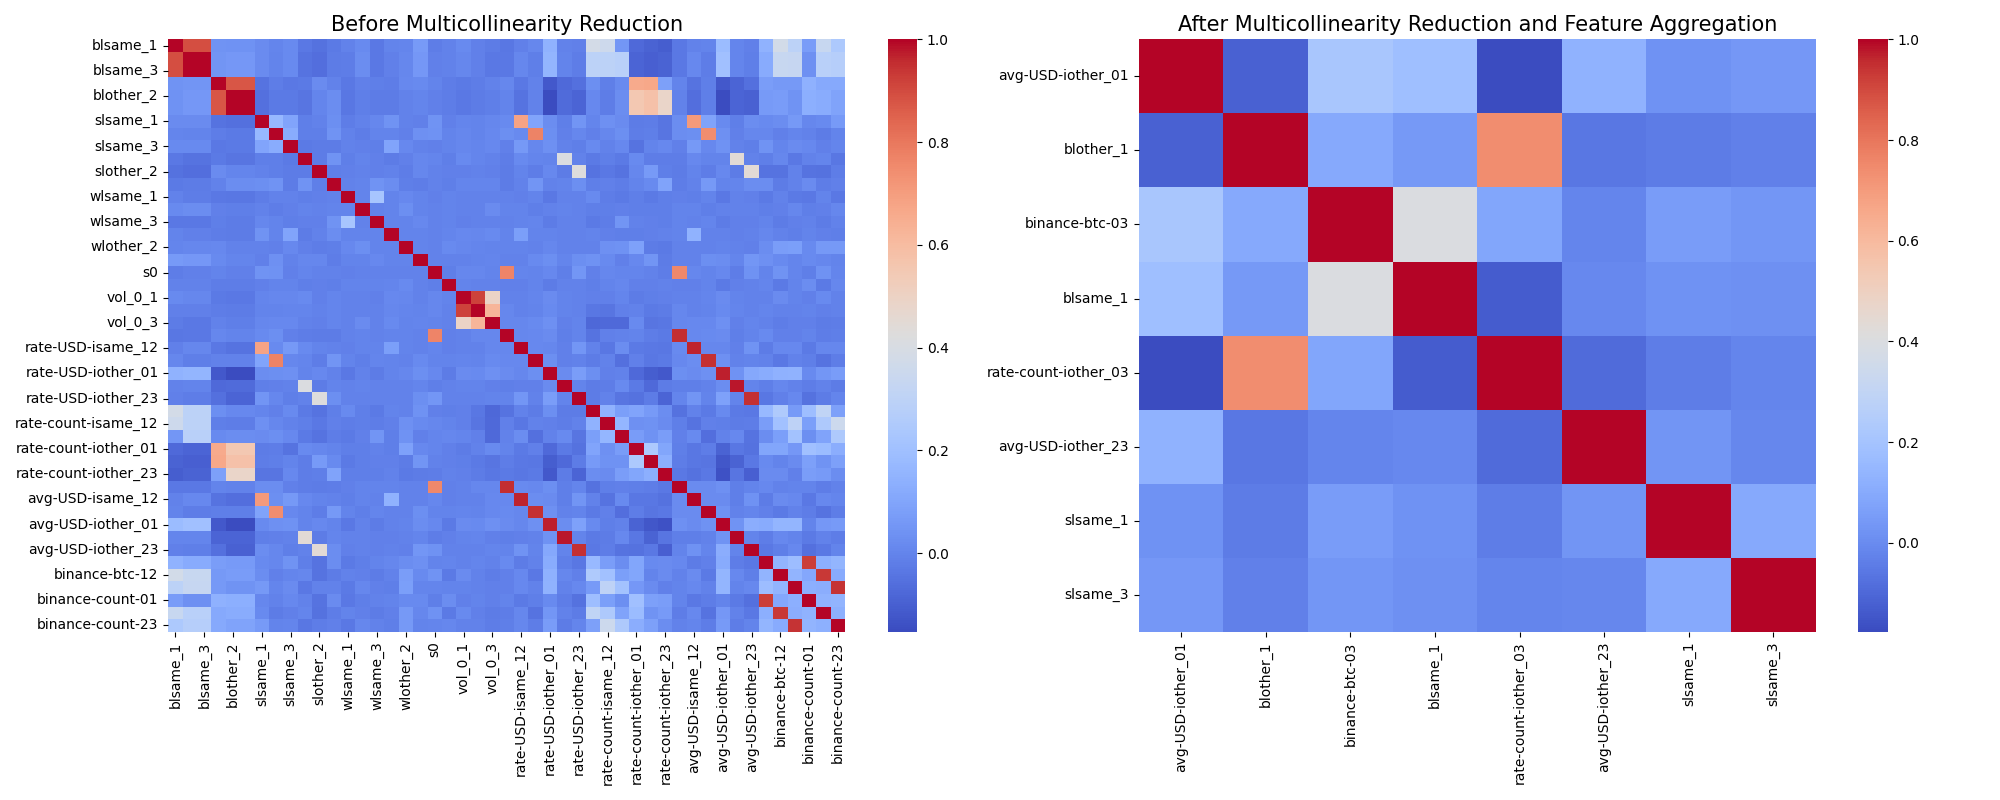
\includegraphics[trim=0 0 0 0, clip, width=0.85\linewidth]{C:/Users/MatiasVizcaino/repos/6203-DataAnalyticsBusiness-Project/Other Resources/correlation_matrix_final.png}
  \caption{Correlation Matrix}
  \label{fig:correlation-matrix}
\end{figure}

\section{\textbf{Feature Selection and Residual Analysis}}

The step-wise feature selection process was used to fit regression models. We systematically removed the least significant features and retrained the model until all remaining features were deemed significant. This approach helps prevent overfitting and enhances model interpretability.


Residual analysis helped inspect the distribution of residuals for any patterns or anomalies. We validated model assumptions: a zero mean error term, constant variance, a normal error distribution, and no correlation between consecutive residuals (autocorrelation). Residuals randomly dispersed around zero signify an appropriate model for the data. If not, it could be a sign that the model's assumptions have been violated.

To identify and address heteroscedasticity, we examine the distribution of error terms. Upon observing a non-linear distribution, we opt to perform a logarithmic transformation using base 10 on the response variables, similar to the approach outlined in \cite{Miori2023}. This transformation aids in stabilizing the variance and aligning the errors with the assumptions of the regression model as illustrated on Figures~\ref{fig:residual-one-horizon} and ~\ref{fig:residual-all-horizons}.

\begin{figure}[htbp]
  \begin{minipage}{0.5\textwidth}
  \centering
  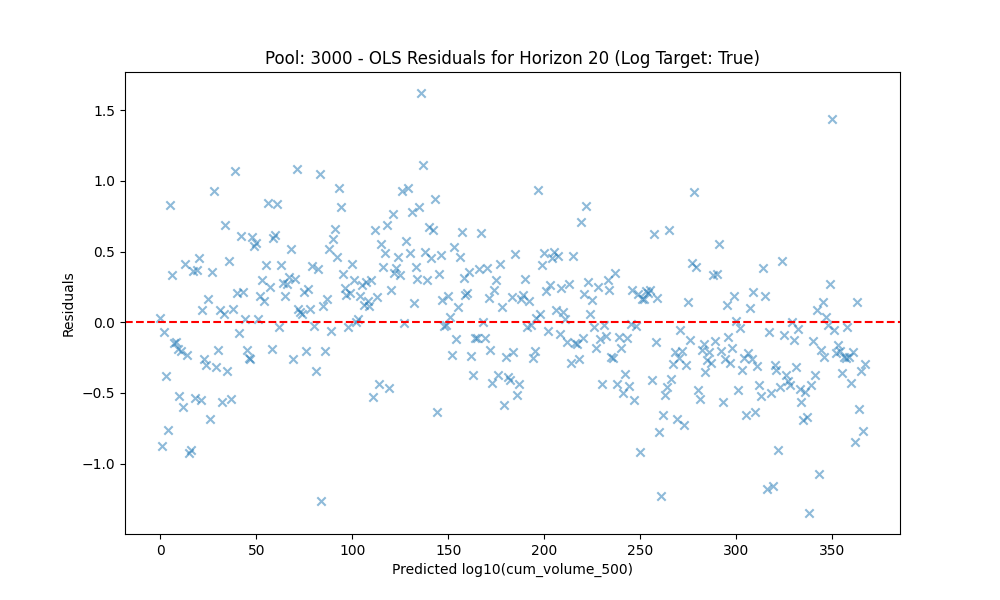
\includegraphics[width=\linewidth]{C:/Users/MatiasVizcaino/repos/6203-DataAnalyticsBusiness-Project/Other Resources/residuals.png}
  \caption{Residuals: One Horizon}
  \label{fig:residual-one-horizon}
  \end{minipage}
  \begin{minipage}{0.45\textwidth}
  \centering
  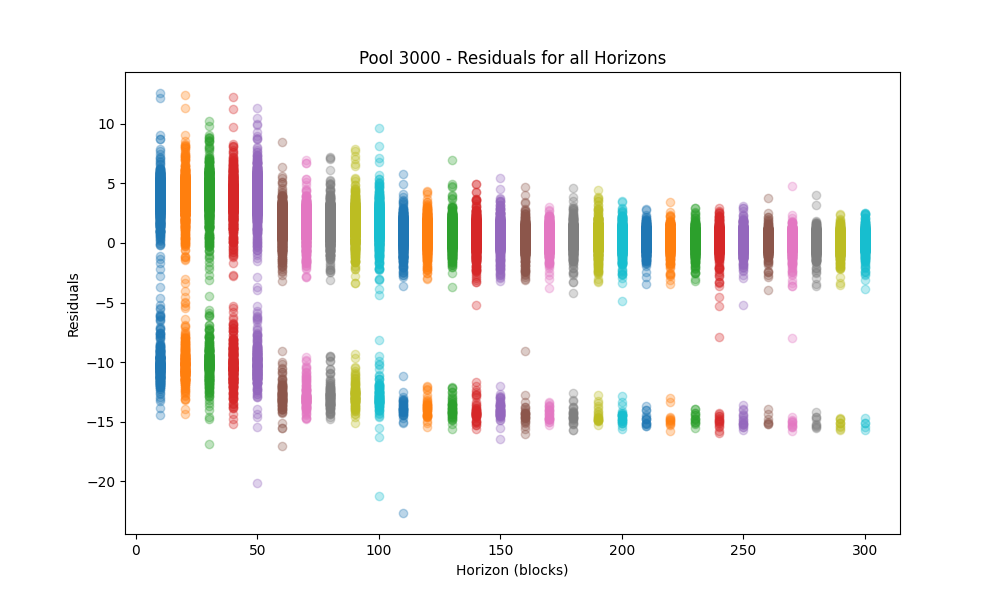
\includegraphics[width=\linewidth]{C:/Users/MatiasVizcaino/repos/6203-DataAnalyticsBusiness-Project/Other Resources/residuals_all_horizons.png}
  \caption{Residuals: All Horizons}
  \label{fig:residual-all-horizons}
  \end{minipage}
  \end{figure}

\subsection{Interpretation of Predictor Coefficients}
When interpreting the predictor coefficients in our OLS regression model for "Best Horizon Run" (using a 'step-wise' model with parameters \texttt{pool = 3000} and \texttt{target\_variable = 'cum\_volume\_500'}), we observe a significant overall relationship (F-statistic = 57.38, p \textless{} 0.001), and an R-squared value of 0.238, indicating that the predictors collectively account for 23.8% of the variance in the dependent variable.

\begin{table}[htbp]
  \centering
  \begin{tabular}{|l|c|c|c|c|}
  \hline
  \textbf{Predictor}        & \textbf{Coef} & \textbf{Std Err} & \textbf{P-value} & \textbf{Significance} \\
  \hline
  Constant                  & 6.1377        & 0.026            & 0.000            & True                  \\
  avg-USD-iother\_01       & 0.1750        & 0.013            & 0.000            & True                  \\
  blother\_1               & -0.1919       & 0.018            & 0.000            & True                  \\
  binance-btc-03          & 0.0976        & 0.013            & 0.000            & True                  \\
  blsame\_1                & -0.0612       & 0.014            & 0.000            & True                  \\
  rate-count-iother\_03    & 0.1115        & 0.019            & 0.000            & True                  \\
  avg-USD-iother\_23       & 0.0294        & 0.012            & 0.016            & True                  \\
  slsame\_1                & 0.0181        & 0.012            & 0.135            & False                 \\
  slsame\_3                & 0.0201        & 0.012            & 0.096            & False                 \\
  \hline
  \end{tabular}
  \caption{Predictor Coefficients}
  \label{tab:predictor-coefficients}
\end{table}

We standardized the features before fitting the model, considering this in the interpretation of the coefficients. The predictor coefficients, as shown in Table ~\ref{tab:predictor-coefficients}, represent the change in the response variable for a one standard deviation change in the corresponding predictor, while holding all other predictors in the model constant. For example, for every one standard deviation increase in 'avg-USD-iother\_01', the logarithm of 'cum\_volume\_500' is expected to increase by 0.1750, assuming all other predictors remain constant.

\subsection{Model Evolution and Detailed Performance Analysis}

Our model's development comprised three distinct stages: an initial stage incorporating all available features, a subsequent phase addressing multicollinearity, and a final stage involving stepwise regression to choose the most statistically significant features.

The model's performance was evaluated based on several criteria: horizon sizes, R-squared values, different data pools, and various target variables. As the horizon extended, predictability, as indicated by \( R^2 \) values, generally decreased, which is consistent with the increased difficulty in predicting further into the future. However, 'all\_features' and 'step-wise' run types with the 'cum\_volume\_300' target variable in the 5000 pool demonstrated consistent high \( R^2 \) values across various horizons, suggesting that our model still exhibited good fit and predictive power even for longer horizons.

Interestingly, we observed negative \( R^2 \) values in some instances, particularly within the test set. This suggests that these models performed worse than a simplistic model based on averages, indicating a potential overfitting issue during the training phase, where the models could not generalize effectively to unseen data.

When comparing the 500 and 3000 pools, the larger pool generally provided higher \( R^2 \) values. This might suggest that having more reference mints in pool 3000 leads to more accurate predictions. Additionally, for both pools, the 'cum\_volume\_500' target variable typically yielded higher \( R^2 \) values, hinting at a stronger correlation with the selected features.

\section{\textbf{Discussion and Conclusion}}

The reduction of multicollinearity had a notable impact on improving our model, as evidenced by the substantial reduction of variables with high Variance Inflation Factor (VIF) values. The final model demonstrated robustness and good predictive power across different time horizons.

The highest coefficient in the model is associated with the \(\widetilde{01}X\) spot lagged variable. This suggests that the immediate past period has the most significant influence on future trading volume, a finding that aligns with established financial theories on market behavior.

Residual analysis revealed a slight trend, with residuals mostly positive for lower predicted values and mostly negative for higher predicted values. This pattern indicates potential underprediction and overprediction, respectively, suggesting room for model refinement.

Our study convincingly demonstrates a substantial relationship between liquidity pool sizes and trading volumes. While some models showed evidence of overfitting, our findings reinforce the potential of pool sizes as a robust predictor of trading volumes in our selected markets. These insights expand the understanding of liquidity pool influence and provide valuable guidance for market participants and future research endeavors.



\subsection{Feature Importance}
[TODO] Understanding the variables contributing significantly to the predictive power of our model can guide feature selection and model refinement. This can be accomplished through permutation importance or coefficient estimates, subject to the model and the specific context.

\section{Going Forward}

To summarize, the learnings from this project, particularly regarding data engineering and feature generation, are substantial. This largely unexplored field of financial technology presents vast opportunities for fresh findings and contributions to the existing body of knowledge. Our initial results are promising, and we're eager to delve into the forthcoming phases of our project, emphasizing model optimization and refining our analysis and conclusions.

The model could potentially be improved further by investigating the variables that still have mid/high VIF after the reduction. They might still have some level of correlation with each other, and additional feature engineering might be helpful. For instance, these variables could be further investigated to understand their correlations, and if they are conveying similar information, one of them could potentially be removed.

It would be valuable to investigate if there are any non-linear relationships between the predictors and the target variable. If such relationships exist, they might not be adequately captured by the linear model. In such a case, using a non-linear model might be beneficial.

Possible next steps could involve investigating the residual errors pattern further and possibly applying some transformation to the target variable or the features.

Our future steps in the modeling phase include:

\begin{itemize}
\item Dataset Splitting: Partitioning the dataset into training and test sets, performing model metrics analysis, and interpretation.
\item Analysis Scope: Examining both Pool 500 and Pool 3000, with a focus on target variables related to volume on the same pool as the reference mint, the other pool, or both.
\item Experimentation: Identifying the optimal combinations of features, horizons, and target variables for accurate predictions.
\item Feature Selection: Using techniques like step-wise or Principal Component Analysis to reduce feature complexity, limit overfitting, and improve interpretability.
\end{itemize}

Our planned experiments include testing different lag lengths, incorporating quadratic features or interaction terms, and accounting for structural breaks, such as the Terra-Luna collapse (May 2022) and the Merge (Sep 2022).

We aspire here or on further work to drive a comprehensive analysis and quantitative discussion on:

\begin{enumerate}[itemsep=0pt, topsep=0pt]
\item The relationship between liquidity pool size and trading volume in BTC-ETH liquidity pools.
\item The influence of the liquidity pool size on the slippage in BTC-ETH trading pairs, considering CEX spillover effects.
\item Impact of BTC-ETH price volatility on trading volume relative to liquidity pool size, focusing on price divergence.
\item Specific periods/events that significantly affect the relationship between BTC-ETH liquidity pool size and trading volume.
\end{enumerate}


While Ordinary Least Squares (OLS) regression is a good starting point, it might be worth exploring other types of models that could better capture the relationships in the data. For example, models that can handle non-linear relationships (e.g., decision trees, neural networks) or models that can account for time-dependence in the data (e.g., ARIMA, state space models) could potentially improve performance.

% Given the negative R^2 values, it might also be worth revisiting the data cleaning and preprocessing steps. Ensuring the quality and correctness of the data is crucial for any machine learning task. 

\section{\textbf{Future Extensions}}
Future extension:

Future extensions may include price divergences in BTC-ETH exchanges and pools, as arbitrage opportunities may also drive activity.

\begin{enumerate}[label=\arabic*. ,itemsep=0pt, topsep=0pt]
\item Direct pool features (2): total value locked (TVL)
\item Network spillover effects (8): trade flow imbalance.
\item Price divergences between the 500 and 3000 pools (2).
\end{enumerate}

[A key concept to understand in this analysis is the notion of impermanent loss. The impermanent loss function for Uniswap v2 liquidity providers is a notable concept to be included in the discussion \cite{Aigner2021}. The role of yield farming protocols, their classification, and their sources of yield are also significant considerations in this analysis \cite{Xu2023}]

\section{Appendix}

From the transaction data, we created 8,228 reference blocks that correspond to each mint operation. These blocks were then used to engineer features to calculate metrics for the same pool and other pools. These features capture data about liquidity pools and calculate metrics such as volatility, traded volume rate, trades count, and average volume. To expand the analysis, we have also included lagged features for the previous three mint operations. Table ~\ref{table:chains} serves as our block reference table.
\begin{table}[htbp]
  \centering
  \small
  \begin{tabularx}{\linewidth}{|X|r|l|l|}
    \hline
    \textbf{pool} & \textbf{reference\_blockNumber} & \textbf{same\_blockNumberChain} & \textbf{other\_blockNumberChain} \\
    \hline
    500 & 14498564 & [14498564, nan, nan, nan] & [14498564, nan, nan, nan] \\
    500 & 14498699 & [14498699, 14498564, nan, nan] & [14498699, nan, nan, nan] \\
    500 & 14499597 & [14499597, 14498699, 14498564, nan] & [14499597, 14499560, 14499457, 14499198] \\
    500 & 14499836 & [14499836, 14499597, 14498699, 14498564] & [14499836, 14499560, 14499457, 14499198] \\
    500 & 14500355 & [14500355, 14499836, 14499597, 14498699] & [14500355, 14500043, 14499560, 14499457] \\
    ... & ... & ... & ... \\
    3000 & 15648981 & [15648981, 15648330, 15648305, 15648187] & [15648981, 15648887, 15648536, 15646933] \\
    3000 & 15649246 & [15649246, 15648981, 15648330, 15648305] & [15649246, 15649243, 15648887, 15648536] \\
    3000 & 15649545 & [15649545, 15649246, 15648981, 15648330] & [15649545, 15649522, 15649347, 15649269] \\
    3000 & 15649565 & [15649565, 15649545, 15649246, 15648981] & [15649565, 15649522, 15649347, 15649269] \\
    3000 & 15649578 & [15649578, 15649565, 15649545, 15649246] & [15649578, 15649522, 15649347, 15649269] \\
    \hline
  \end{tabularx}
  \caption{Block Interval Chains}
  \label{table:chains}
\end{table}

Finally, we've constructed a base table \ref{tab:horizon} with the \texttt{start\_blockNumber} of each horizon and the \texttt{reference\_blockNumber}, defined by mint operations in the block. This base table is joined with the mint aggregated transaction data to generate our target variables and independent variables that are lagged.

\begin{table}[htbp]
  \centering
  \small
  \begin{tabular}{cccccc}
    \hline
    \textbf{horizon\_blockNumber} & \textbf{min\_flag} & \textbf{reference\_blockNumber} & \textbf{horizon\_label} & \textbf{cum\_volume\_500} \\
    \hline
    108757 & 0 & 15552674 & 9 & 423,485.34 \\
    108758 & 0 & 15552674 & 10 & 423,485.34 \\
    108759 & 1 & 15552772 & 1 & 328,338.73 \\
    108760 & 0 & 15552772 & 2 & 406,084.78 \\
    108761 & 0 & 15552772 & 3 & 536,640.71 \\
    ... & ... & ... & ... & ... \\
    109047 & 0 & 15555464 & 12 & 122,730.73 \\
    109048 & 0 & 15555464 & 13 & 123,650.59 \\
    \hline
  \end{tabular}
  \caption{Example: Horizon Table (reference mint on pool=3000)}
  \label{tab:horizon}
\end{table}


% The correlation between BTC-ETH liquidity pool size and trading volume: We can infer that larger pool sizes generally result in higher trading volume based on the model performance. The models with larger pool sizes tend to have higher R-squared values, indicating better performance in predicting trading volumes. However, this is an inference and may not be an accurate reflection of the actual correlation. From the predictor coefficients, we can observe that the 'avg-USD-iother_01' variable has a positive coefficient of 0.1750, which is statistically significant. This suggests that an increase in the average traded volume on the WBTC-WETH pools (over the 01 block range) leads to a positive impact on the cumulative volume in the reference pool. This provides some evidence of a positive relationship between pool size (represented indirectly by the average traded volume) and trading volume in the reference pool.

The effects of BTC-ETH price volatility on trading volume compared to liquidity pool size: The binance-btc-03 predictor in your OLS model, which you've stated represents spillover effects from Binance, could potentially encapsulate aspects of price volatility. Its positive coefficient suggests that as these spillover effects (which may include price volatility) increase, the dependent variable also increases.

% \textbf{Adapting Mathematical Formulas:} We adapted the formulas from the Uniswap v3 liquidity math paper for calculating impermanent loss and changes in holdings after a price change. This adaptation helped us demonstrate P&L calculations and provided a deeper understanding of Uniswap's dynamic \cite{Elsts2021} .

Time-Series Specific Analysis: If your data has a temporal component, consider analyzing autocorrelation and partial autocorrelation plots of the residuals. This will help you check for any leftover temporal structure in your errors which, if present, suggests there may be room to improve your model.

These insights from the residual analysis can guide further refinement of the models. For example, exploring different models or additional features for smaller horizons could improve prediction accuracy.


In conducting this macroeconomic study, we acknowledge and address various challenges and risks associated with decentralized finance (DeFi) protocols. One of the main challenges lies in understanding and managing the economic risks inherent in yield farming, including yield dilution, conversion risk, exchange risk, counterparty risk, and liquidation risk. These risks can have significant implications for the sustainability and effectiveness of yield farming practices within the DeFi ecosystem \cite{Xu2023}.

Furthermore, we recognize the importance of addressing security risks in our analysis. Flash loan attacks, rug pulls, reentrancy vulnerabilities, and key exploits are prevalent security risks within the yield farming landscape. Mitigating these risks and ensuring the security of DeFi protocols are crucial for maintaining the stability and integrity of the overall system \cite{Xu2023}.

\bibliographystyle{plain} % You could use plain, unsrt, alpha, abbrv etc. 
\bibliography{export}

\end{document}